\section{Обзор предметной области}

\subsection{Постановка задачи}

Задача генерации речи имеет простую математическую формулировку. По заданному отрывку текста со строковым представлением (конечная последовательность символов из конечного алфавита), сгенерировать аудиодорожку с хорошо слышимой человеческой речью соответствующей заданному отрывку. Формат аудио обычно представляет из себя последовательность из 16-битных действительных чисел от $-1.0$ до $1.0$ -- дискретное приближение непрерывной аудиоволны. Основной параметр такого формата - это частота дискретизации, выражаемая в герцах (Гц, Hz). Популярными частотами для аудио отрывков в системах генерации речи являются $22.05$ кГц и $24$ кГц (22050 и 24000 значения в секунду соответственно). Чем выше частота дискретизации -- тем лучше качество аудио (так как лучше приближение), но тем сложнее уловить зависимости для генерации (Рисунок~\ref{fig:sample-rate}).

\begin{figure}[!ht]
\centering
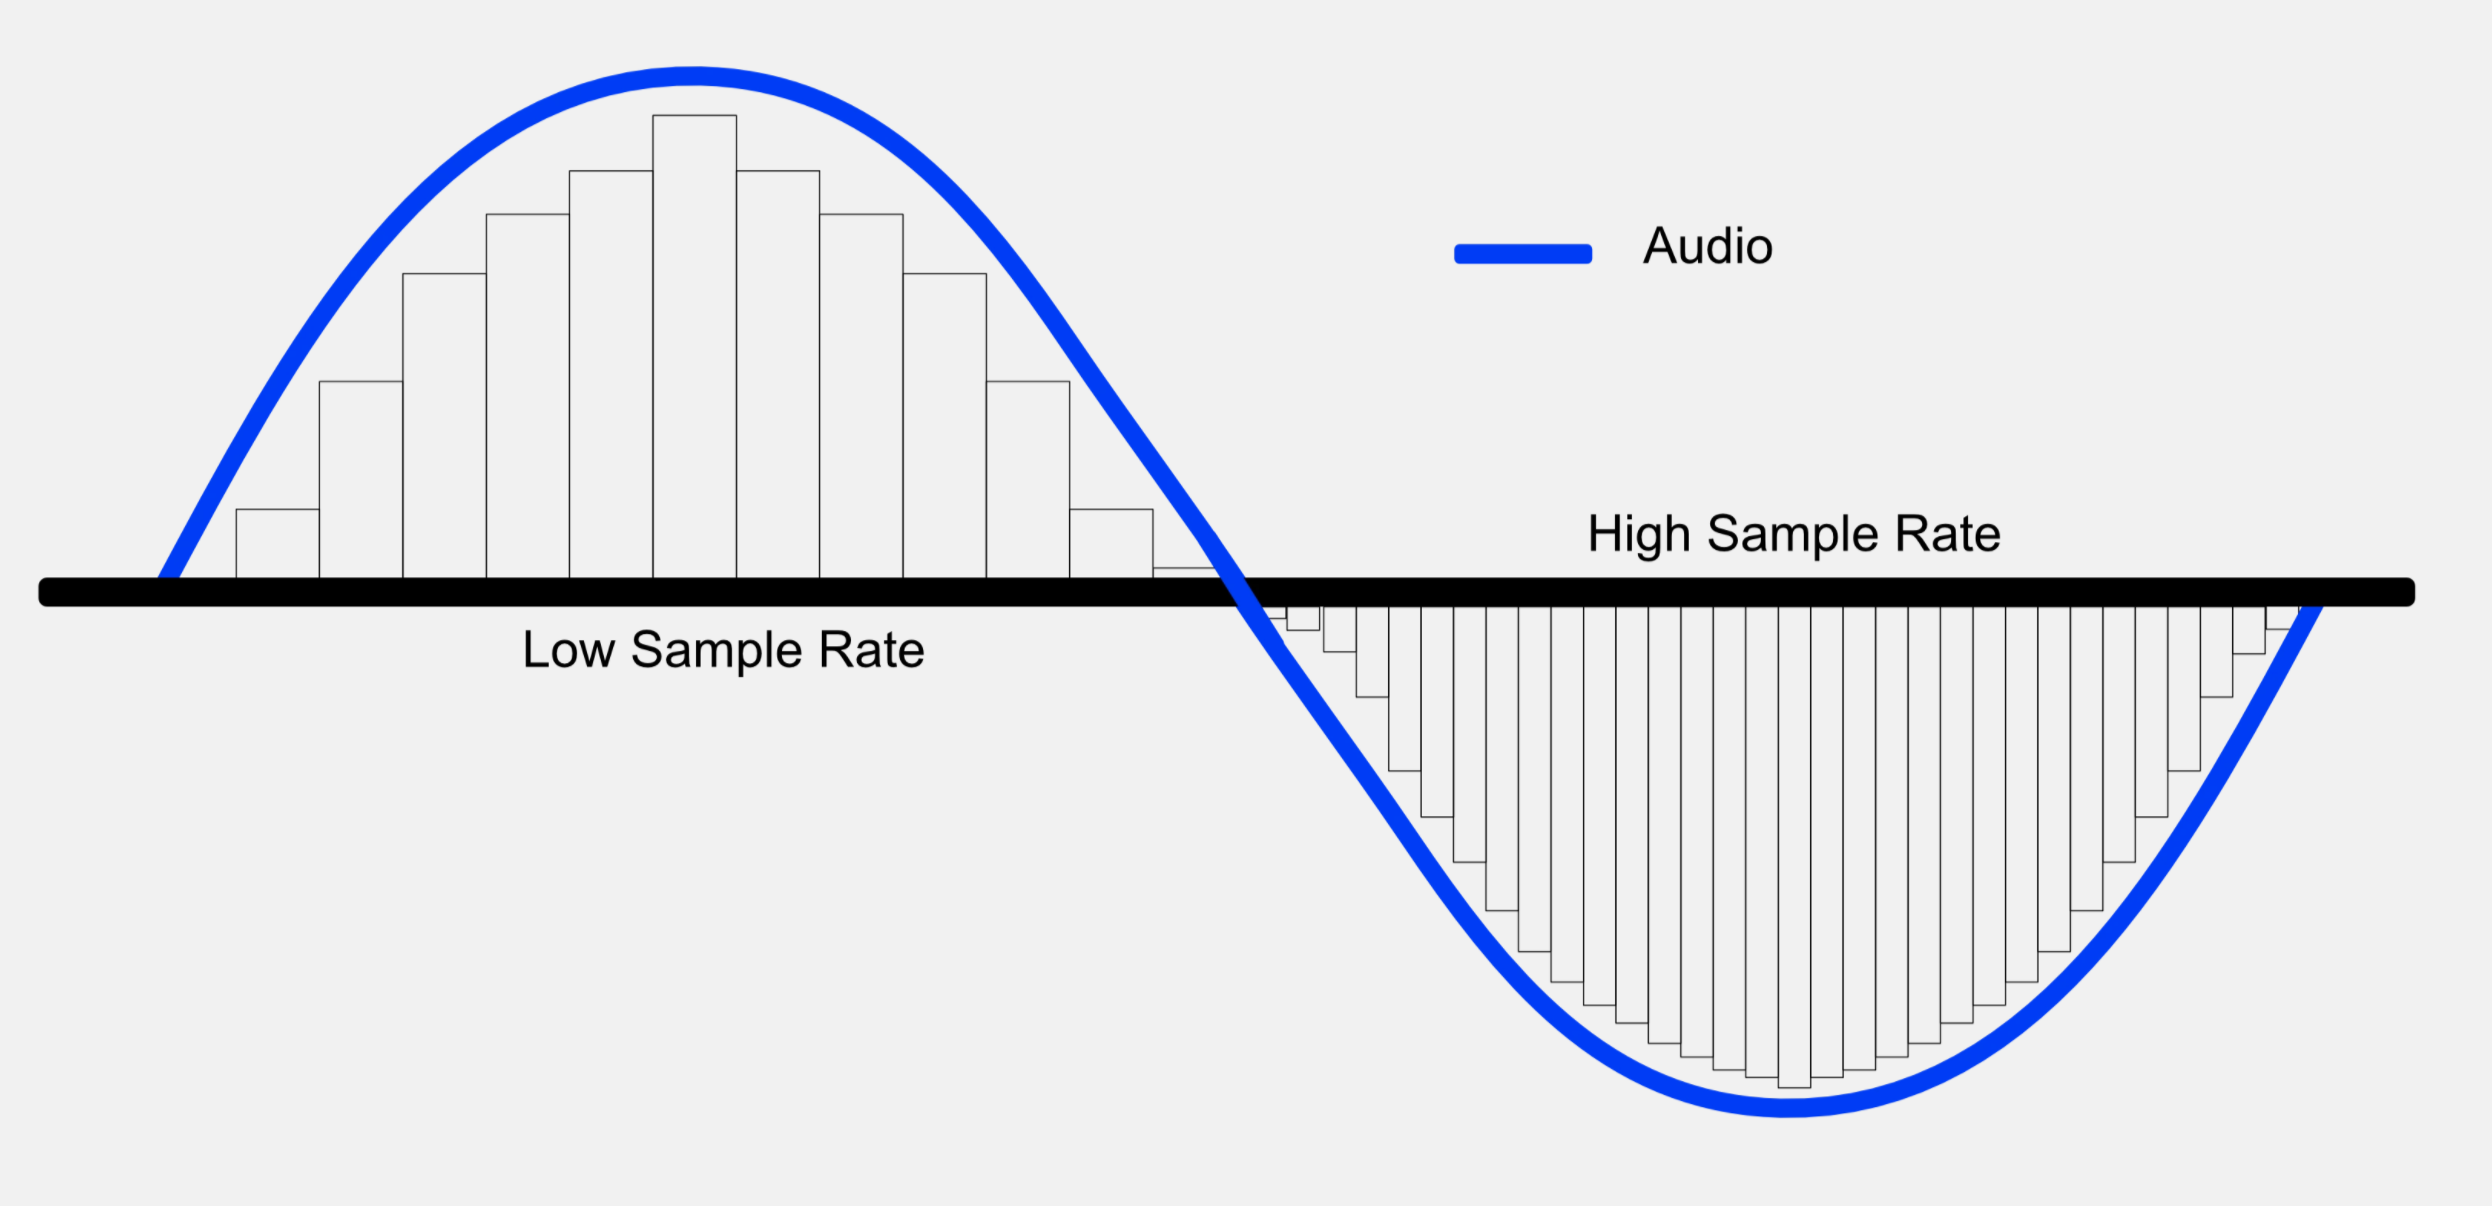
\includegraphics[width=1.0\textwidth]{images/sample-rate.png}
\caption{Примеры различной частота дискретизации (sample rate) для представления аудио}
\label{fig:sample-rate}
\end{figure}

Модели на основе нейронных сетей (NN) для преобразования текста в речь (Text-To-Speech, TTS) превзошли как конкатенативный (concatenative), так и статистический параметрический подходы для синтеза речи с точки зрения качества. Они также значительно упрощают процесс синтеза речи. Традиционно. системы синтеза речи объединяет несколько блоков: модель для извлечения лингвистических признаков из текста, модель предсказания длительности, модель предсказания акустических признаков и вокодер на основе обработки сигналов~\cite{taylor}, который служит для преобразования акустических признаков в аудиодорожку. Нейронные TTS системы, как правило, имеют два этапа (Рисунок~\ref{fig:tts-pipeline}). На первом этапе модель генерирует мэл-спектрограммы из текста. На втором этапе вокодер на основе нейронной сети синтезирует речь из мэл-спектрограмм. Большинство моделей TTS на основе нейронных сетей имеют архитектуру encoder-decoder~\cite{bahdanau} с операциями с механизмом внимания (attention), которые, как было замечено, имеют некоторые общие проблемы:
\begin{enumerate}
    \item Тенденция повторять или пропускать слова~\cite{fastspeech}, из-за сбоев работы механизма внимания, когда некоторые подпоследовательности повторяются или игнорируются. Для решения этой проблемы модели, основанные на механизме внимания, используют дополнительные правила поощрения монотонного внимания~\cite{tacotron2, deepvoice3, taigman2017}. В общем же случае, механизм внимания часто ведет к проблемам на этапа вывода, а также замедляет скорость обучения, так как обычно состоит как минимум из одной операции с квадратичной по времени асимптотикой.
    \item Медленная скорость вывода относительно параметрических моделей.
    \item Нет простого способа контролировать просодию (паттерн ритма и интонации голоса) или скорость голоса, так как длина генерируемой последовательности определяется декодером.
\end{enumerate}

\begin{figure}[!ht]
\centering
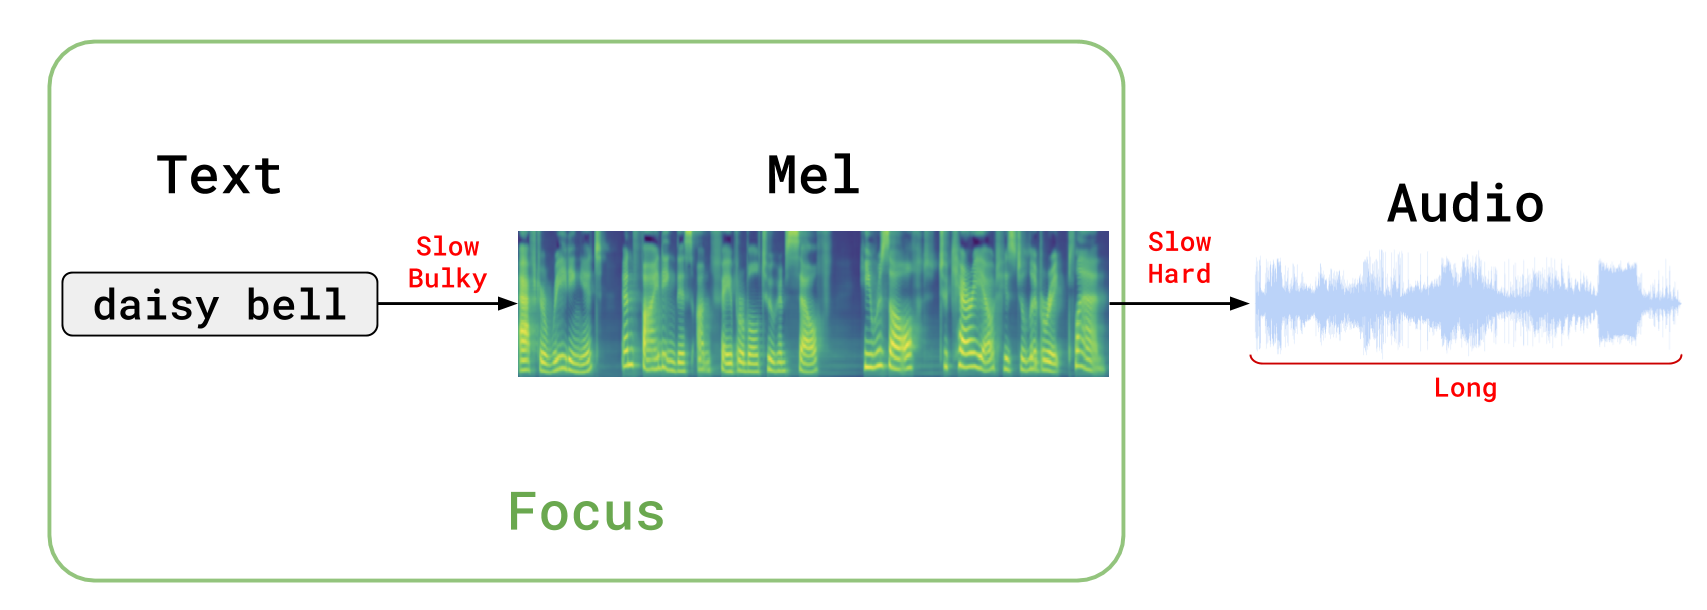
\includegraphics[width=1.0\textwidth]{images/tts-pipeline.png}
\caption{Два шага TTS систем. Первый шаг -- генерация мэл-спектрограммы -- будет рассматриваться в рамках данной работы. Второй шаг -- вокодинг -- отдельная сложная задача. Оба шага имеют полно нерешенных проблем: медленная скорость работы, большое количество весов, заметно уступающее качество в сравнении с записью человеческой речи.}
\label{fig:tts-pipeline}
\end{figure}

\subsection{Особенности предлагаемого подхода}

В рамках данной работы описывается новая нейронная модель TTS для решения проблем описанных выше. Модель состоит из двух сверточных сетей. Первая сеть предсказывает длительности графем (входных символов). Далее, входной текст расширяется, повторяя каждый символ в соответствии с предсказанной длительностью. Вторая сеть генерирует мэл-спектрограммы из развернутого текста. Наконец, используется вокодер WaveGlow~\cite{waveglow} для синтеза звука из мэл-спектрограмм (Рисунок~\ref{fig:arch}). Финальная часть -- вокодер -- не является частью модели и должна рассматриваться в рамках отдельной задачи, но в данной работе будет использоваться WaveGlow из-за наличия универсальной претренированой модели и возможности сравнения с другими подходами.

\begin{figure}[!ht]
\centering
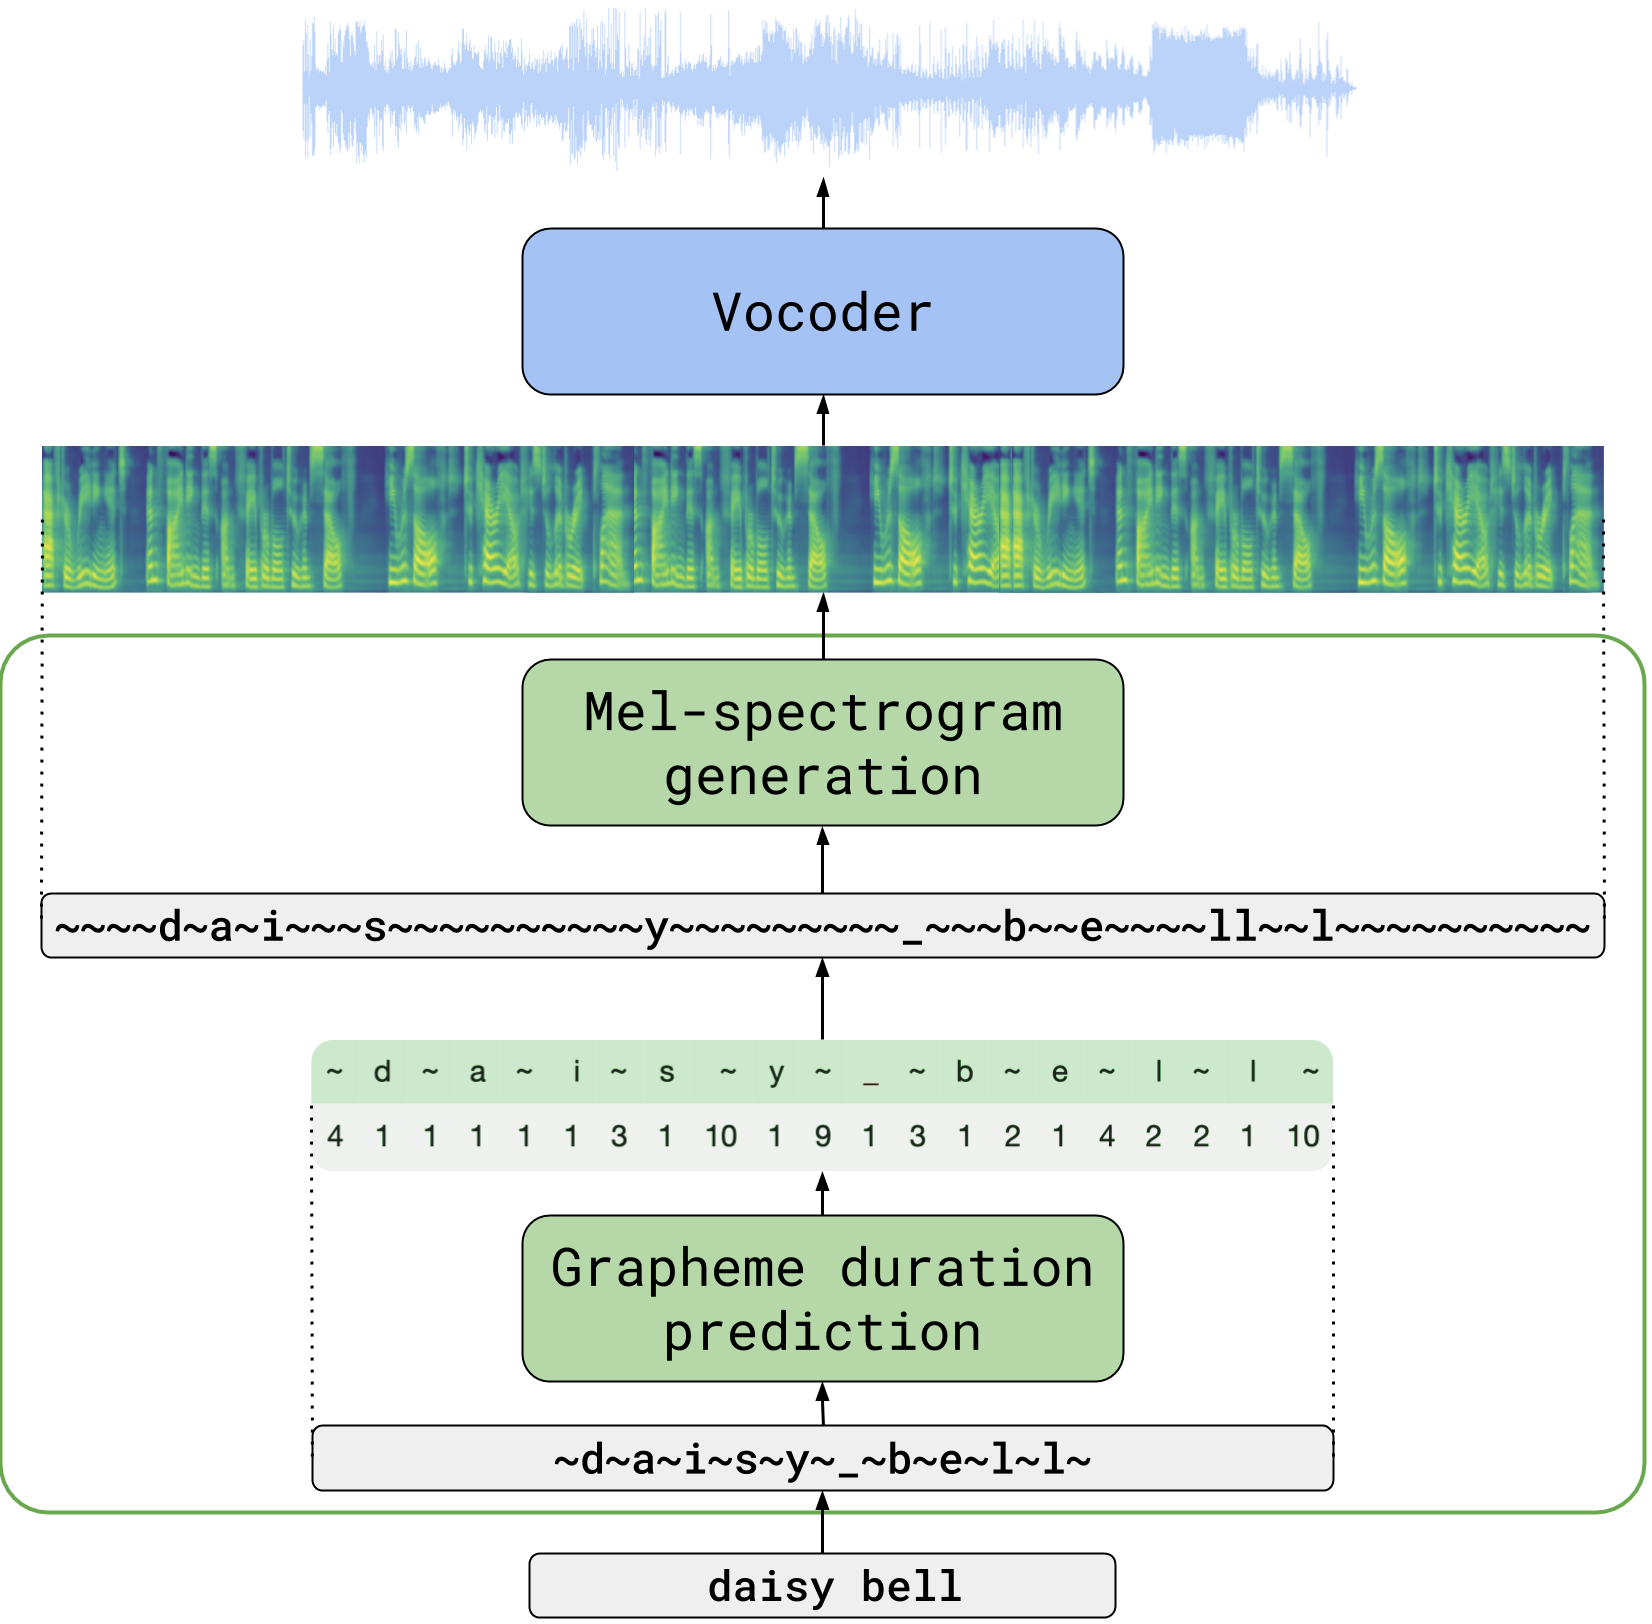
\includegraphics[width=1.0\textwidth]{images/arch.png}
\caption{TalkNet преобразует текст в речь, используя предиктор длительностей графем, генератор мэл-спектрограмм и вокодер. $\sim$ используется в рамках данной работы для обозначения пустого символа из выхода CTC функции ошибки.}
\label{fig:arch}
\end{figure}

Чтобы обучить предсказатель длительностей графем, нам нужно сначала получить истинное выравнивание между входными символами и звуковой дорожкой по времени. Аналогичная проблема выравнивания существует в автоматическом распознавании речи (ASR), которая решается явным образом с помощью Connectionist Temporal Classification (CTC)~\ref{fig:ctc}. CTC маргинализирует вывод по всем возможным выравниваниям, выбирая наилучшее. Выбирая наиболее вероятный выход в каждый момент времени, его можно использовать его для выравнивания между входным звуком и выходным текстом. Это выравнивание не является совершенным, и в нем могут быть ошибки. В рамках данной работы показано, что если модель ASR точна и имеет низкую частоту ошибок в символах (Char-Error-Rate, CER), то можно извлечь достаточно хорошее выравнивание между текстом и звуком. Полученное выравнивание на основе CTC можно применить для обучения модели, которая будет предсказывать длительности графем для входного текста. Предиктор длительности графемы заменяет выравнивание на основе механизма внимания (attention) и позволяет избежать пропуски и повторения слов. При этом. эксперименты с набором данных LJSpeech~\cite{ljspeech} показывают, что качество речи для TalkNet сравнимо с лучшими авторегрессионным подходами.

Конволюционная структура обоих частей позволяет проводить параллельное обучение, также значительно ускоряет скорость вывода. Такая структура позволяет работать значительно быстрее со значительно меньшим числом параметров, поддерживая качество генерируемой речи аналогичное FastSpeech~\cite{fastspeech} и Tacotron 2~\cite{tacotron2}.

\subsection{Обзор методов генерации речи}

Методы синтеза речи, основанные на статистике, обычно имеют следующие части: преобразователь графем в фонемы, предиктор длительностей фонемы, генератор акустических признаков (например, мэл-спектрограмм) и вокодер~\cite{taylor}. Zen et al~\cite{zen2009,zen-2015,zen-2016} предложили гибридную нейронную параметрическую модель TTS (Рисунок~\ref{fig:stats-tts} и \ref{fig:zen-tts}), в которой глубокие нейронные сети используются для прогнозирования длительности фонемы и генерации акустических признаков на уровне кадра. Предиктор длительности фонемы был обучен на основе скрытой марковской модели (HMM), из которой извлекались фонетические выравнивания.

\begin{figure}[!ht]
\centering
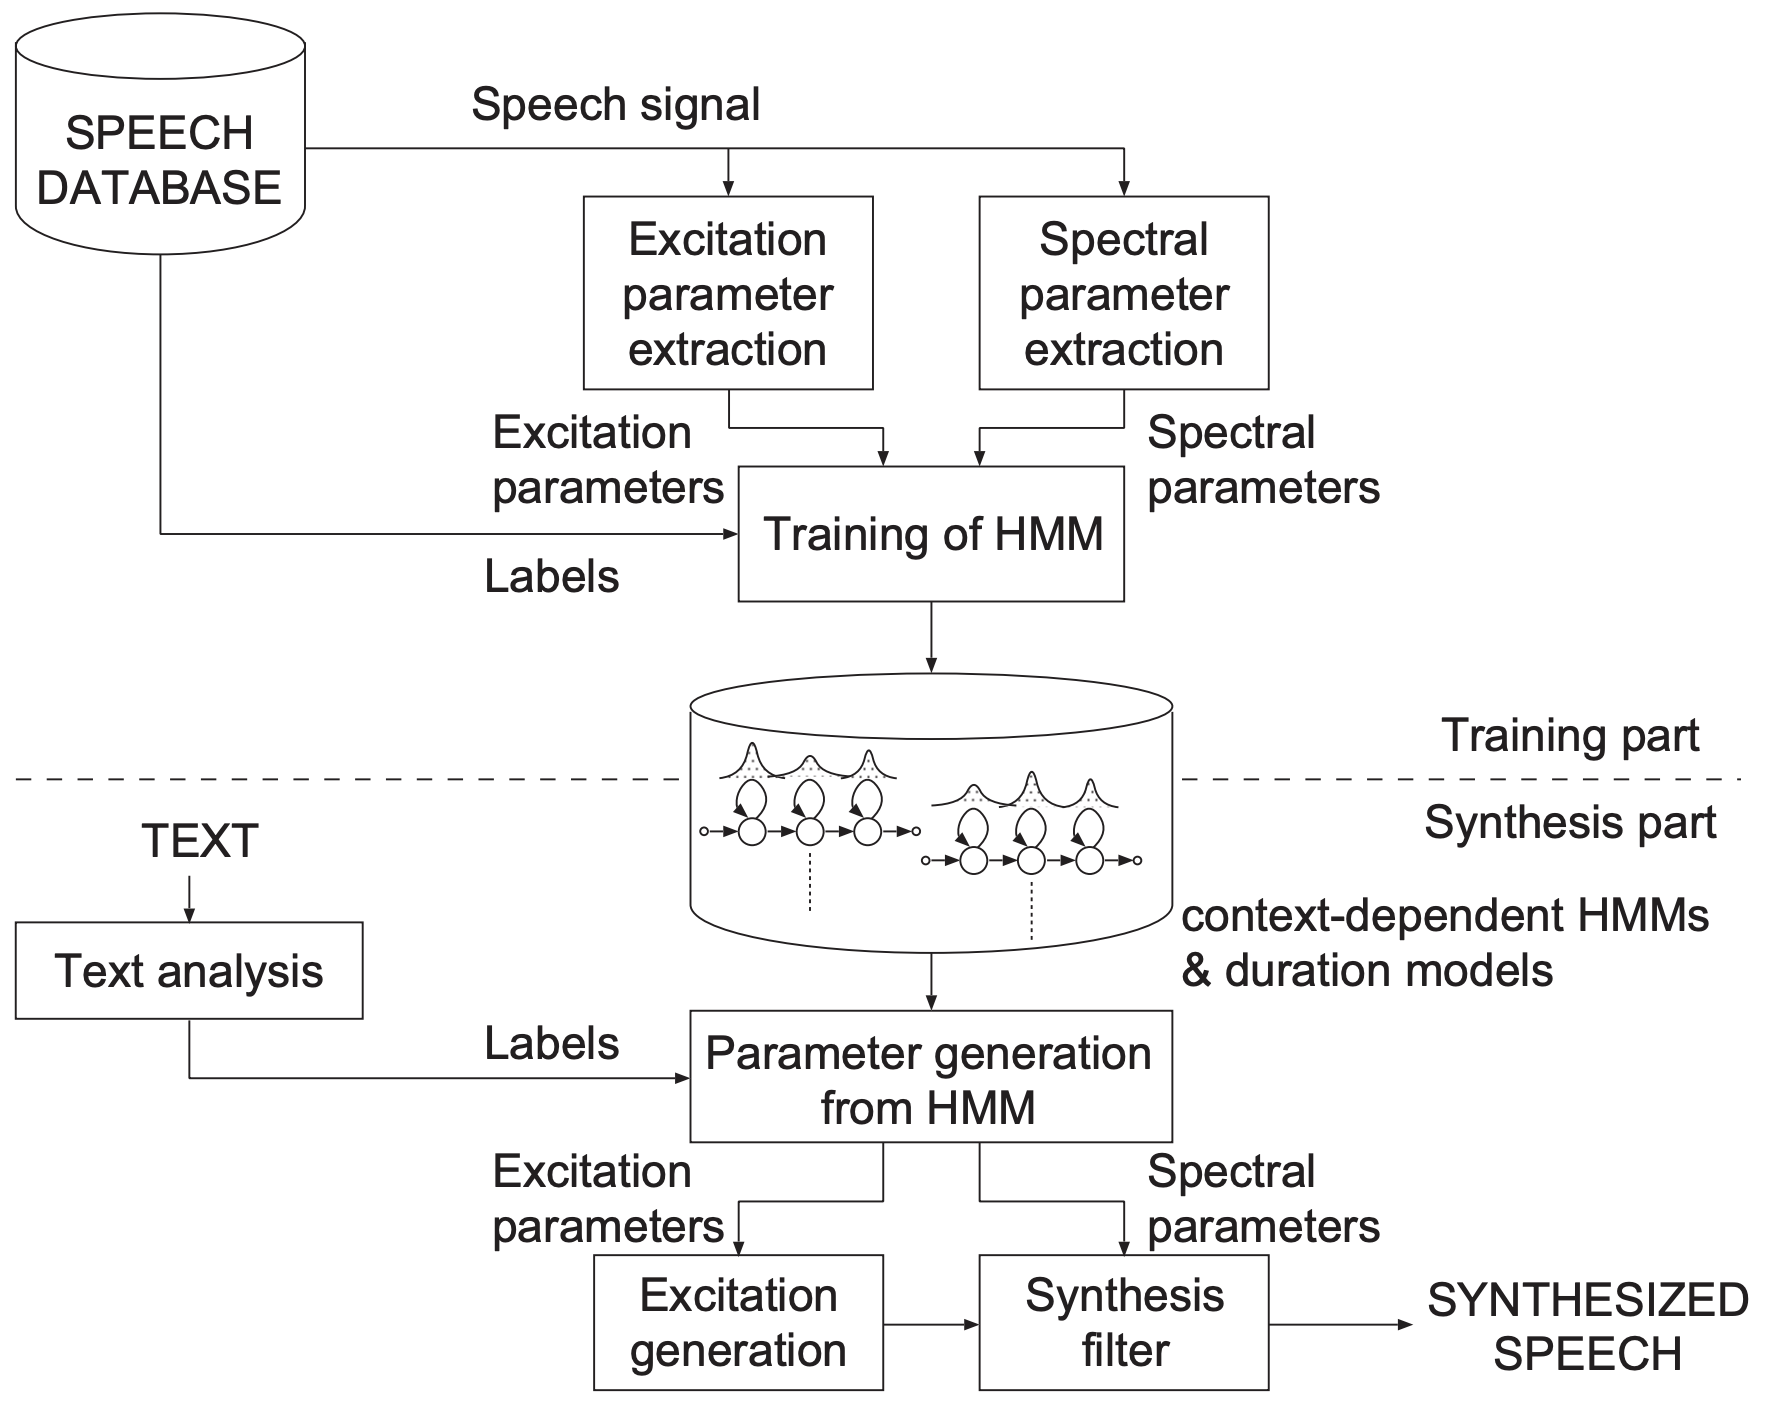
\includegraphics[width=1.0\textwidth]{images/related-work/stats-tts.png}
\caption{Блок-диаграмма работы статистической TTS системы с предсказанием длительностей графем~\cite{zen2009}}
\label{fig:stats-tts}
\end{figure}

\begin{figure}[!ht]
\centering
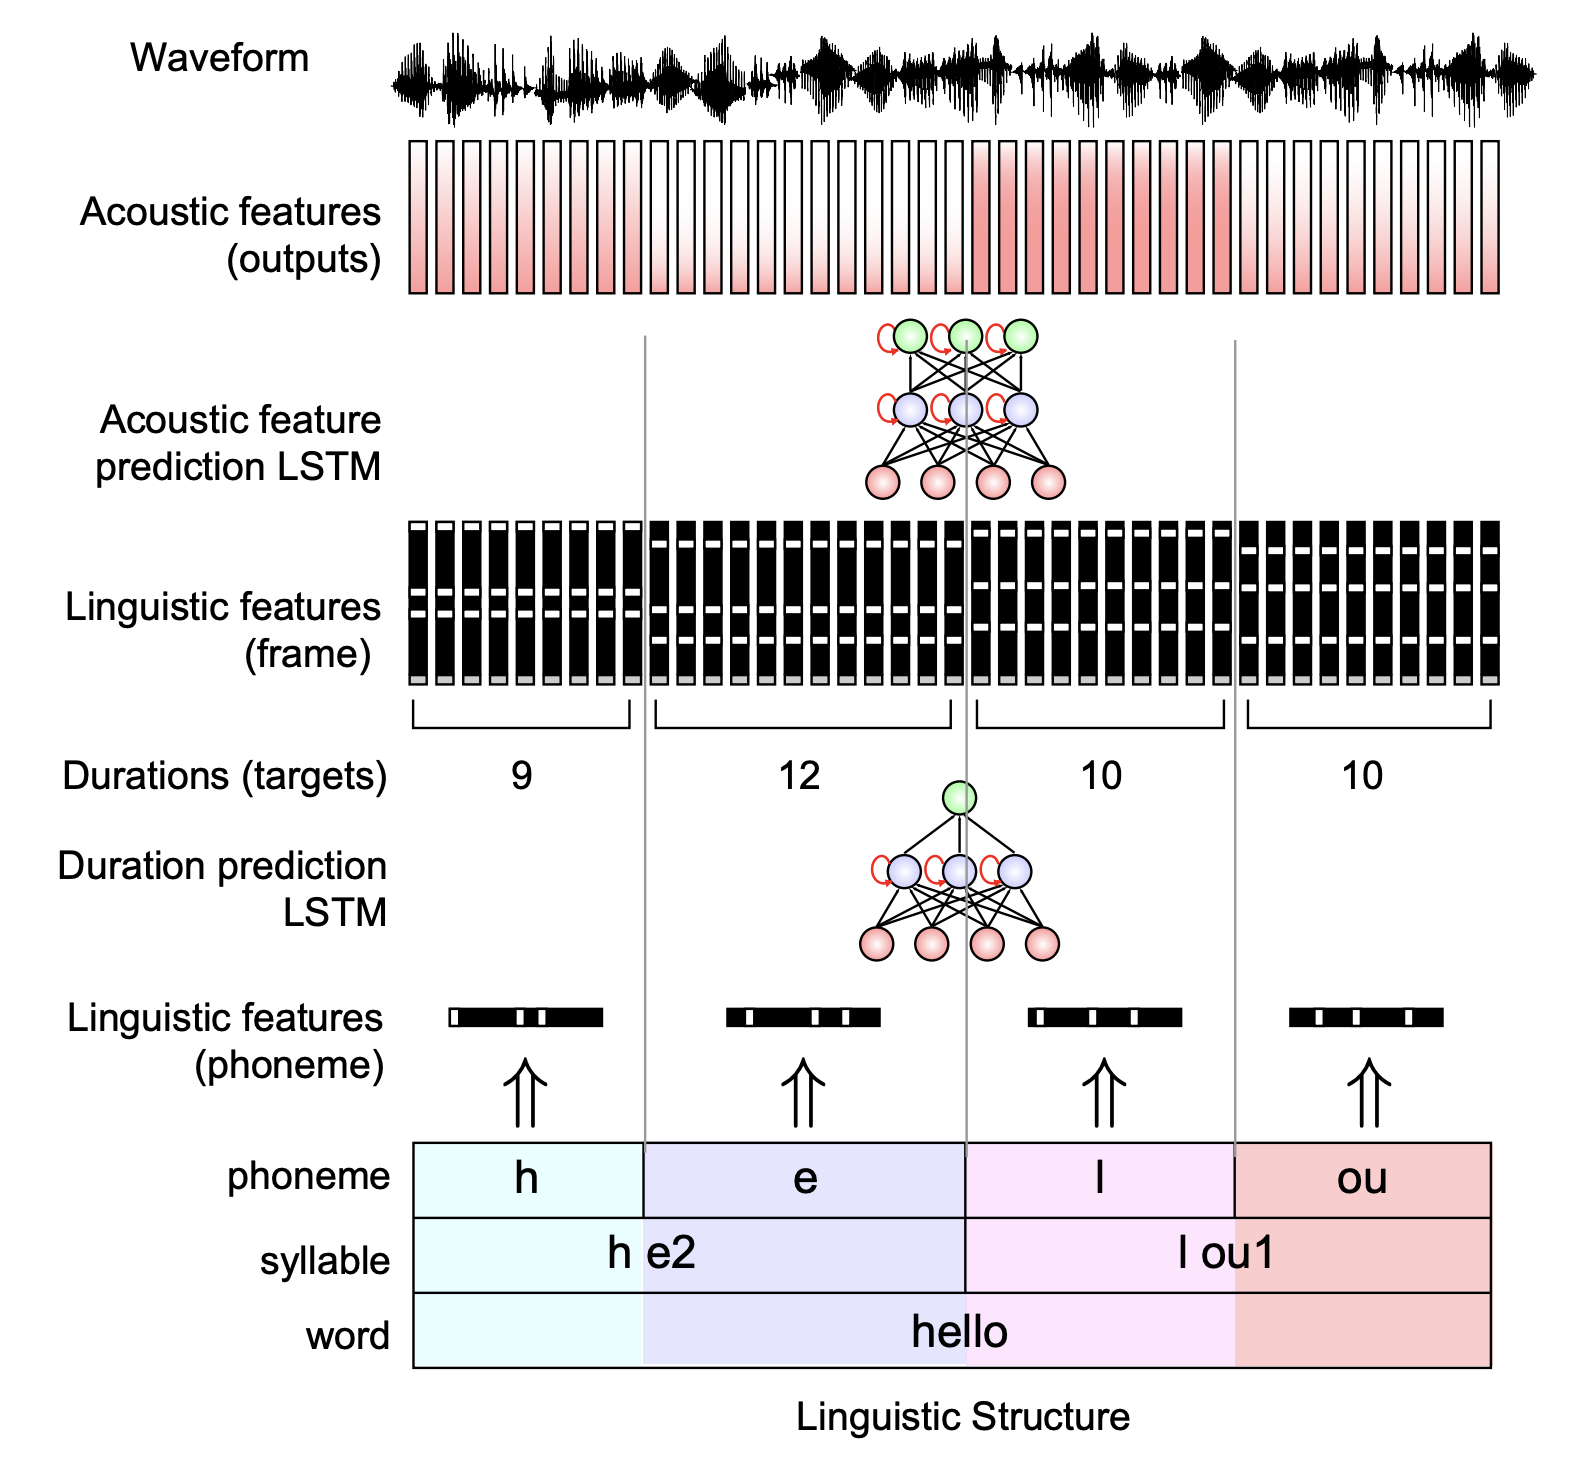
\includegraphics[width=1.0\textwidth]{images/related-work/zen-tts.png}
\caption{Более современный вариант модели с предсказыванием длительностей входных графем с использованием нейронных сеток~\cite{zen-2015,zen-2016}}
\label{fig:zen-tts}
\end{figure}

Один из других возможных подходов -- DeepVoice~\cite{deepvoice1, deepvoice2} (Рисунок~\ref{fig:related-work:deepvoice-1} и \ref{fig:related-work:deepvoice-2}) -- также основан на для традиционной для области синтеза речи структуре, но заменяет обучаемые компоненты на нейронные сети. Для обучения предиктора длительности фонем была использована вспомогательная модель на основе CTC для фонетической сегментации, позволяющая аннотировать данные по границам фонем. Другая модель -- Tacotron~\cite{tacotron1,tacotron2} (Рисунок~\ref{fig:related-work:tacotron-2}) -- это end-to-end нейронная сеть, которая принимает символы в качестве входных данных и сразу выводит мэл-спектрограмму слева направо шаг за шагом (авторегрессионно). Tacotron 2 использует архитектуру encoder-decoder с механизмами внимания. Encoder состоит из трех сверточных слоев и одного двунаправленного LSTM. Decoder представляет собой рекуррентную нейронную сеть (RNN) с чувствительным к местоположению монотонным вниманием (location-sensitive monotonic attention). Авторегрессионность Tacotron2 позволяет хорошо учитывать контекст, а механизмы внимания позволяют правильно расставлять акценты при произношении. Tacotron2 -- одна из лучших на сегодняшний день моделей по качеству, однако для ее обучения требуется много времени (до нескольких дней).

\begin{figure}[!ht]
\centering
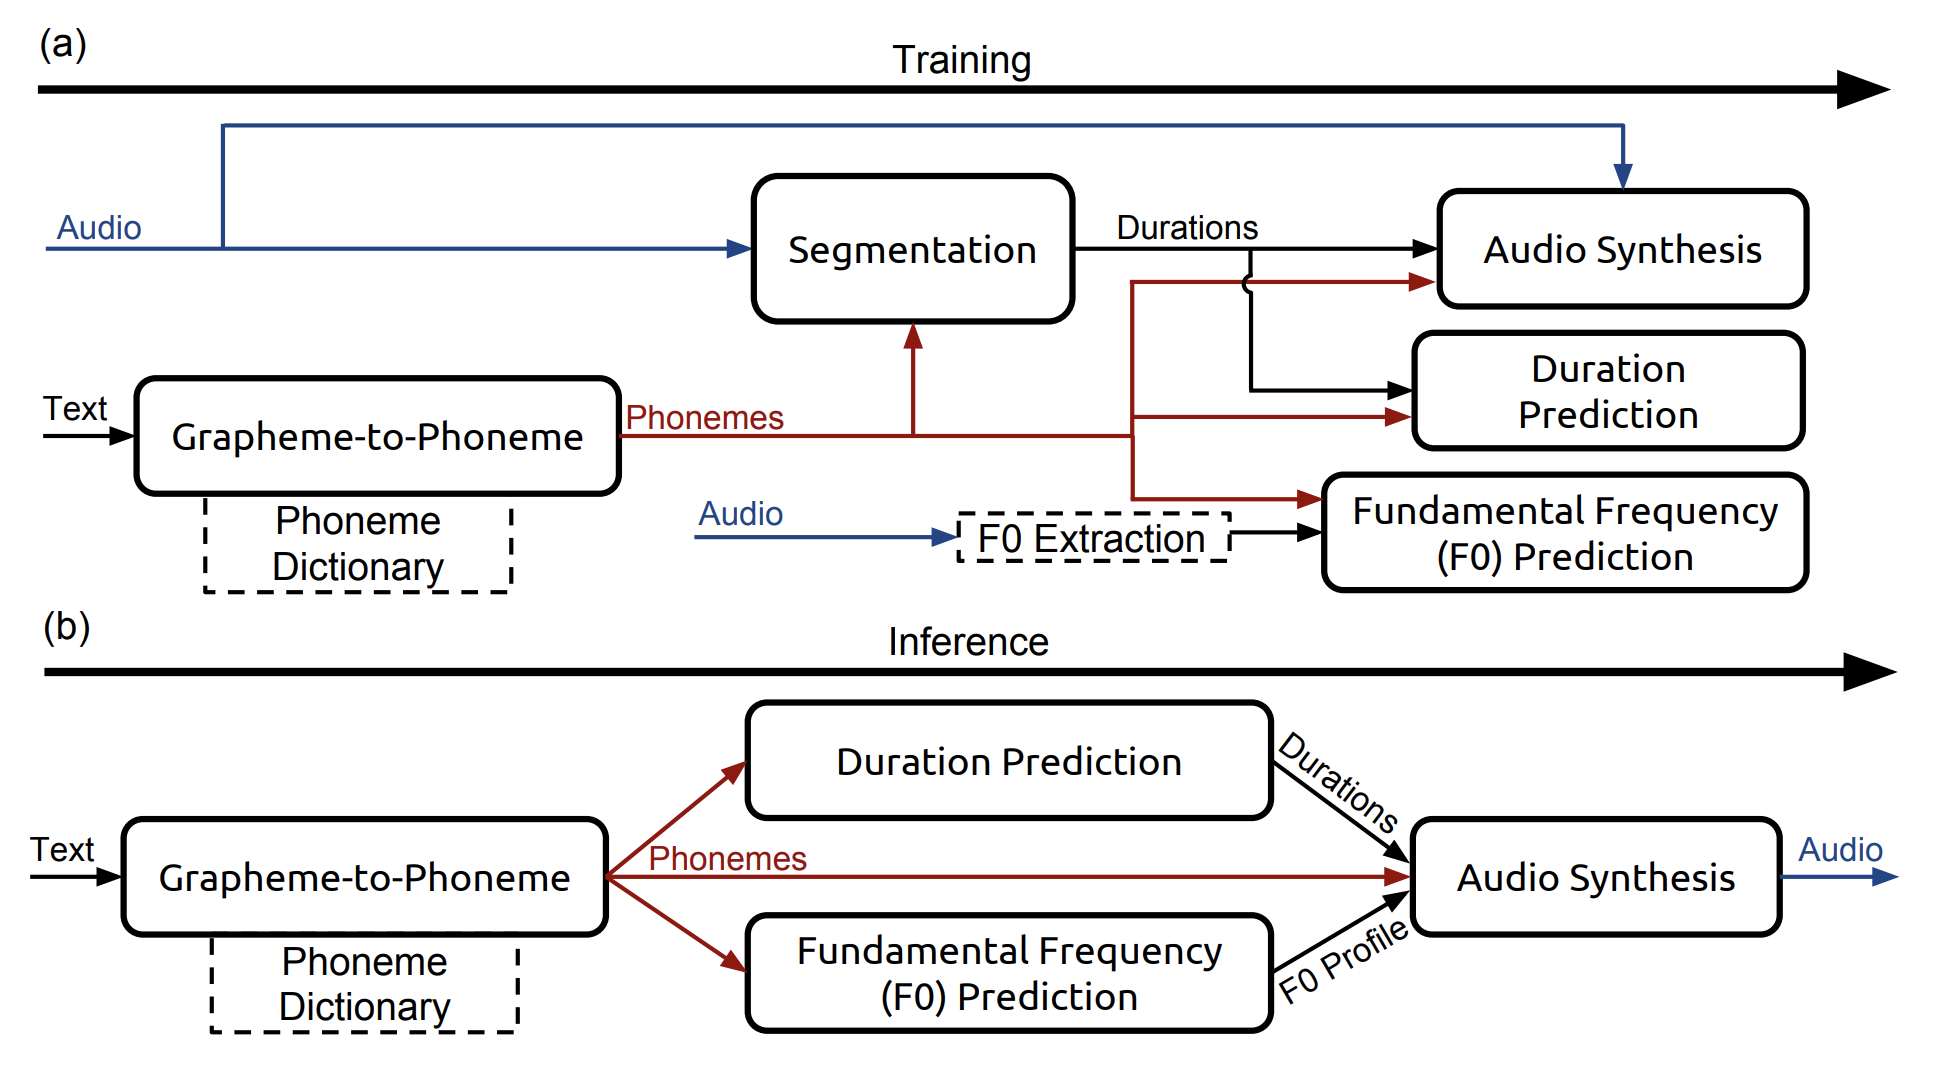
\includegraphics[width=1.0\textwidth]{images/related-work/deepvoice-1.png}
\caption{Диаграмма описывающая модель DeepVoice1~\cite{deepvoice1} с промежуточным шагов в виде предсказания длительностей}
\label{fig:related-work:deepvoice-1}
\end{figure}

\begin{figure}[!ht]
\centering
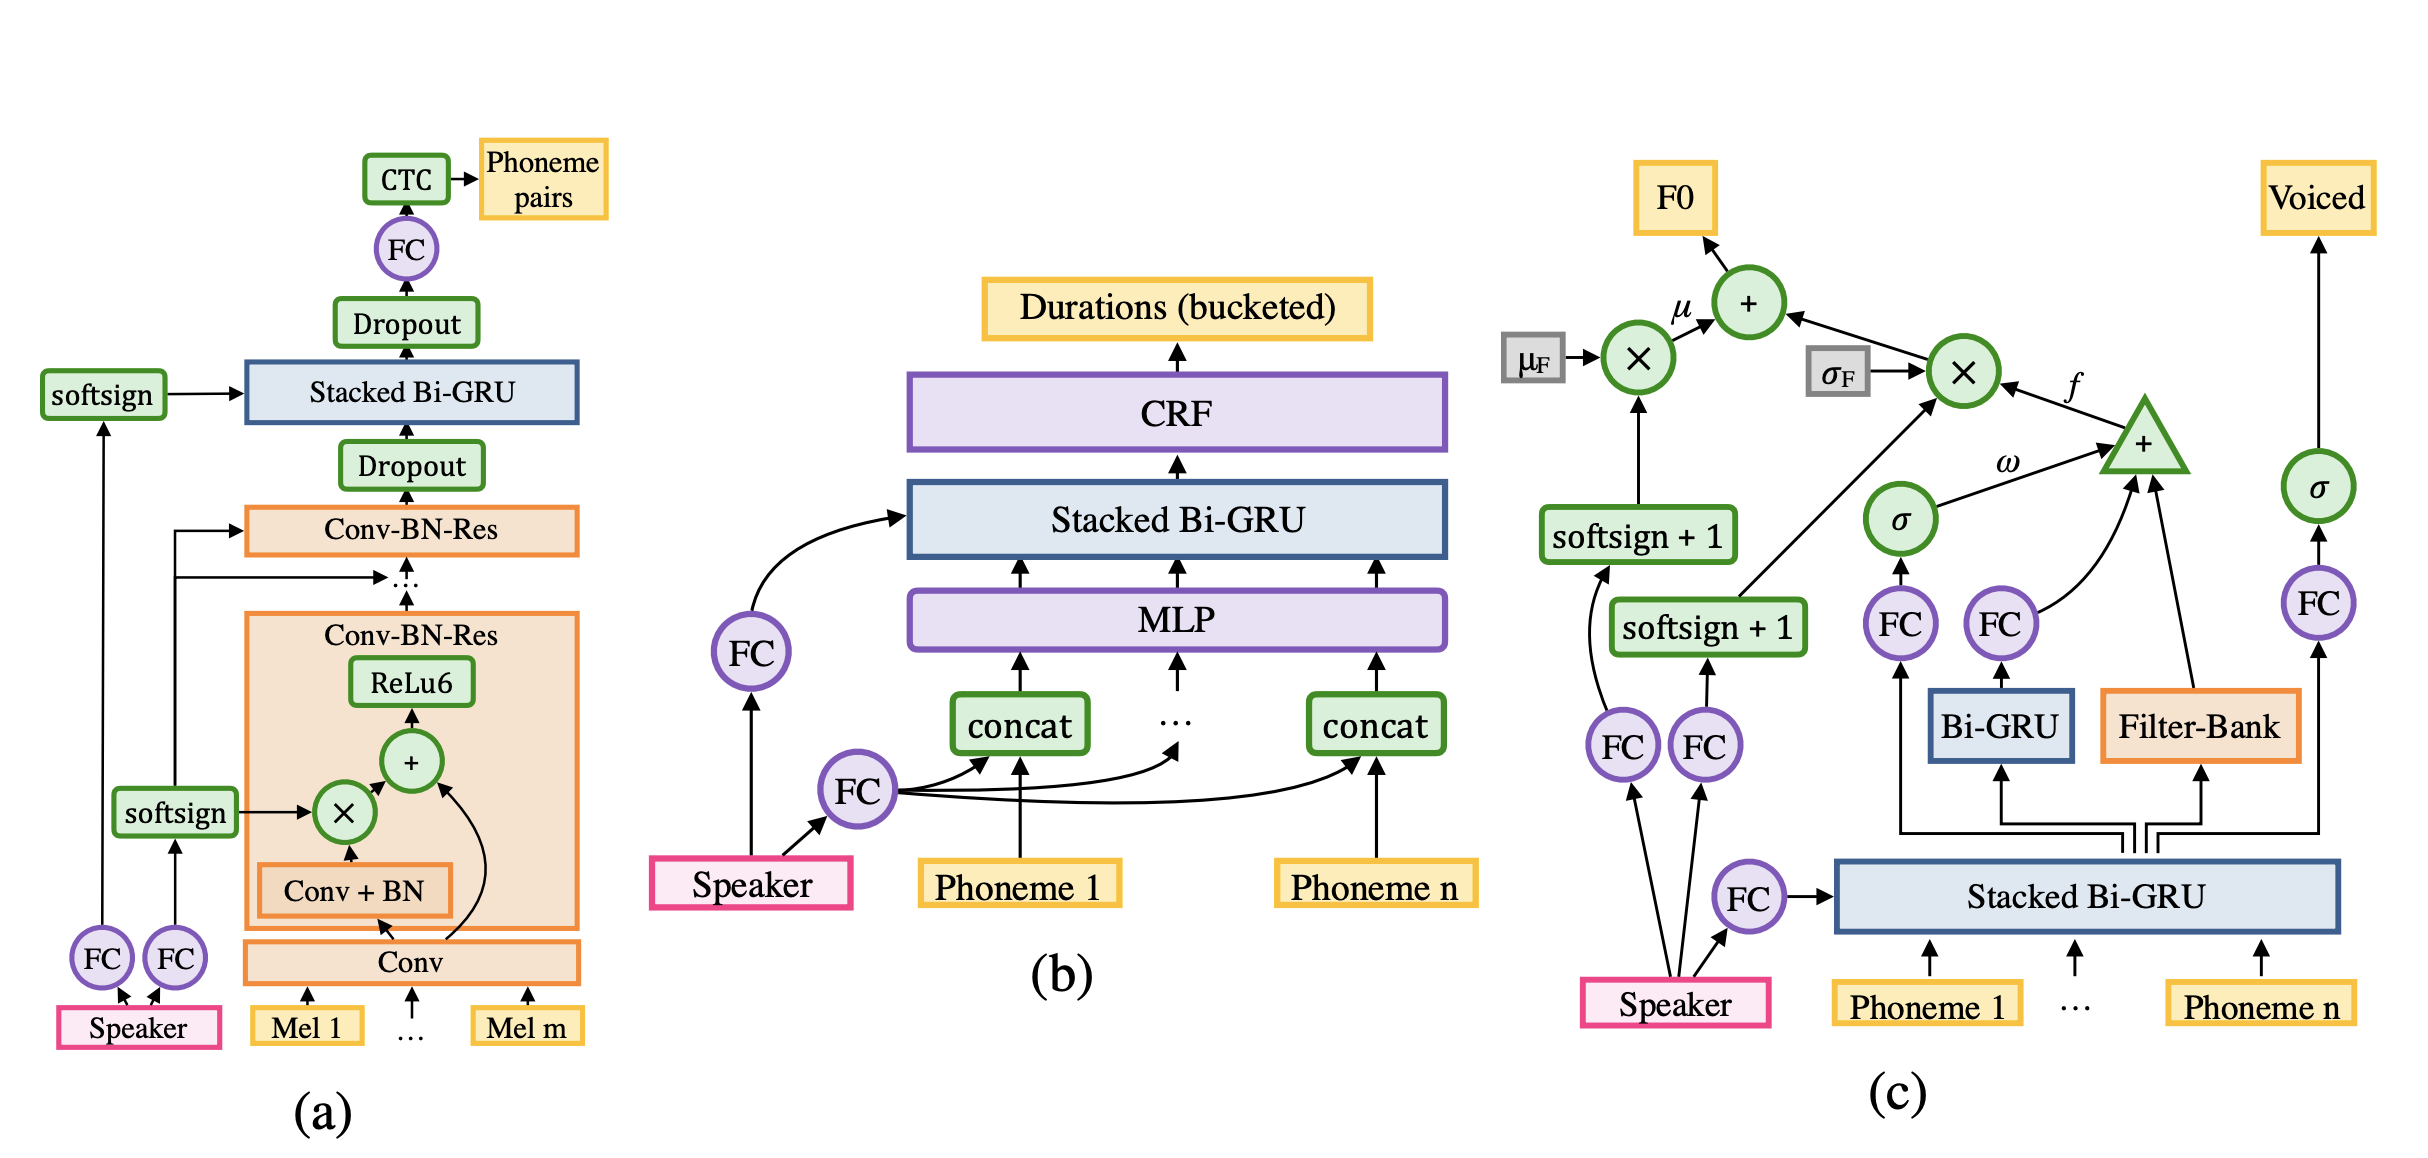
\includegraphics[width=1.0\textwidth]{images/related-work/deepvoice-2.png}
\caption{DeepVoice2 с multi-speaker расширением}
\label{fig:related-work:deepvoice-2}
\end{figure}

\begin{figure}[!ht]
\centering
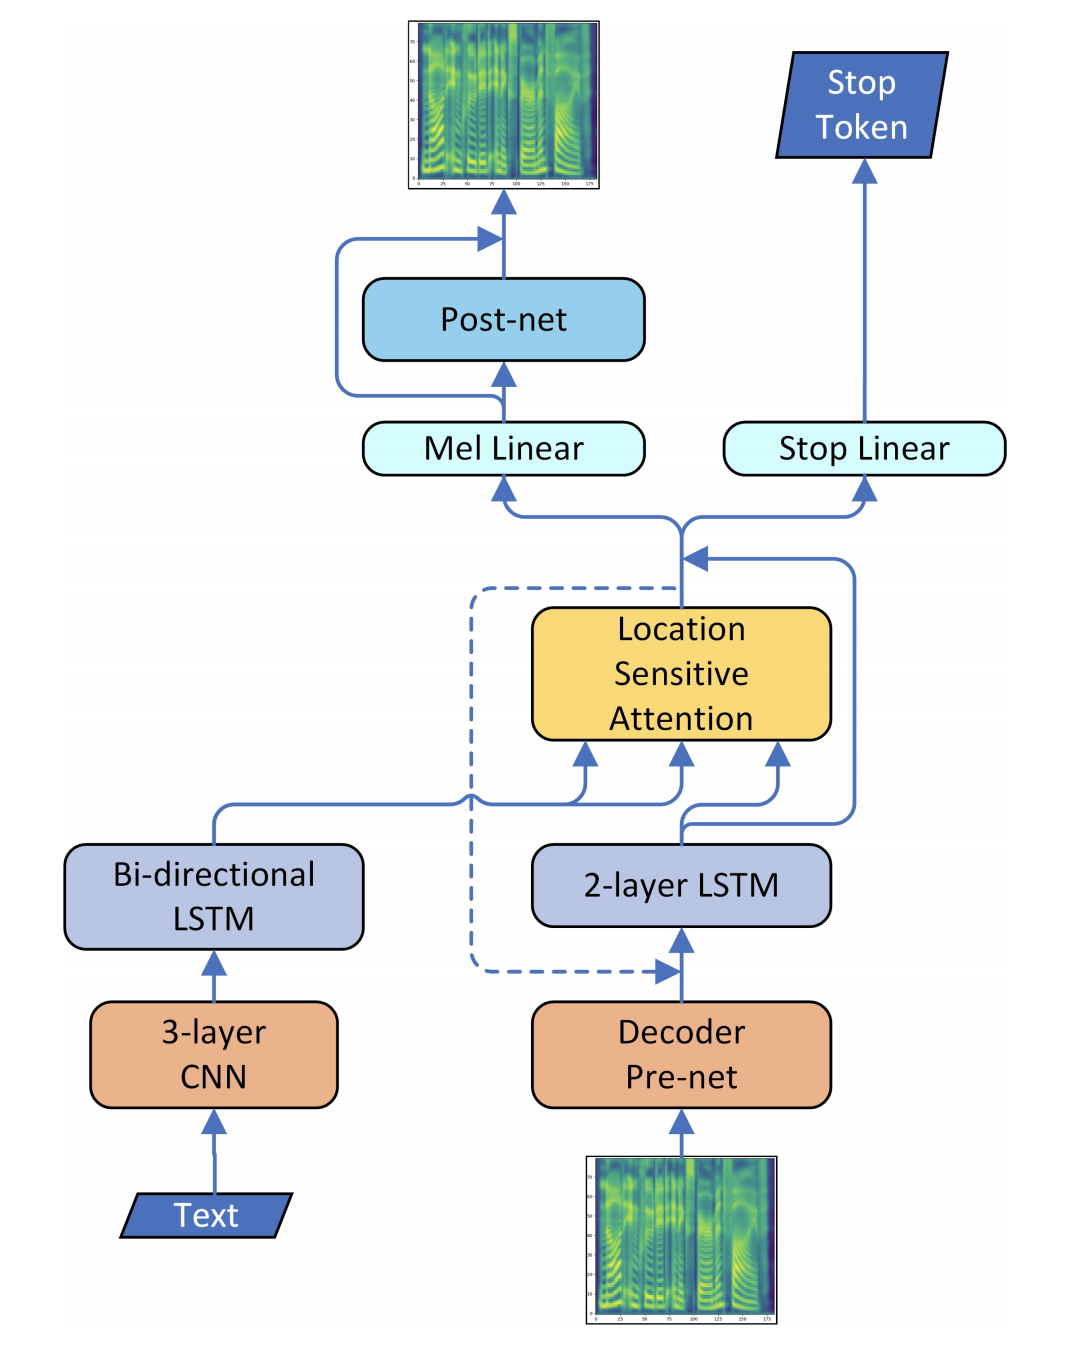
\includegraphics[width=0.7\textwidth]{images/related-work/tacotron-2.png}
\caption{Процесс генерации речи для авторегрессионного Tacotron2}
\label{fig:related-work:tacotron-2}
\end{figure}

Последовательный характер моделей на основе рекуррентных нейронных сетей (RNN) ограничивает эффективность обучения и вывода. Но для генерации речи не обязательно использовать RNN. DeepVoice 3~\cite{deepvoice3} (Рисунок~\ref{fig:related-work:deepvoice-3}) заменяет RNN на конволюционную модель с encoder-decoder архитектурой и монотонным механизмом внимания. Переход от RNN к сверточной нейронной сети (CNN) ускоряет обучение, но вывод модели по-прежнему является авторегрессионным. Другой end-to-end моделью TTS, которая не использует RNN, является ParaNet~\cite{paranet} (Рисунок~\ref{fig:related-work:paranet}). ParaNet -- это еще одна конволюционная encoder-decoder с механизмом внимания. Для обучения ParaNet требуется другая предобученная TTS модель, у которой заимствуется матрица внимания. Наконец, Transformer-TTS и~\cite{transformer-tts} (Рисунок~\ref{fig:related-work:transformer-tts}) заменяет рекуррентные нейронные сети с encoder-decoder структурой на трансформеры~\cite{attention-is-all} (модель, основанная на применении механизма внимания несколько раз подряд). Transformer-TTS сначала преобразует текст в фонемы с помощью конвертера на основе правил. Используя последовательности фонем в качестве входных данных, Transformer-TTS генерирует мэл-спектрограмму.

\begin{figure}[!ht]
\centering
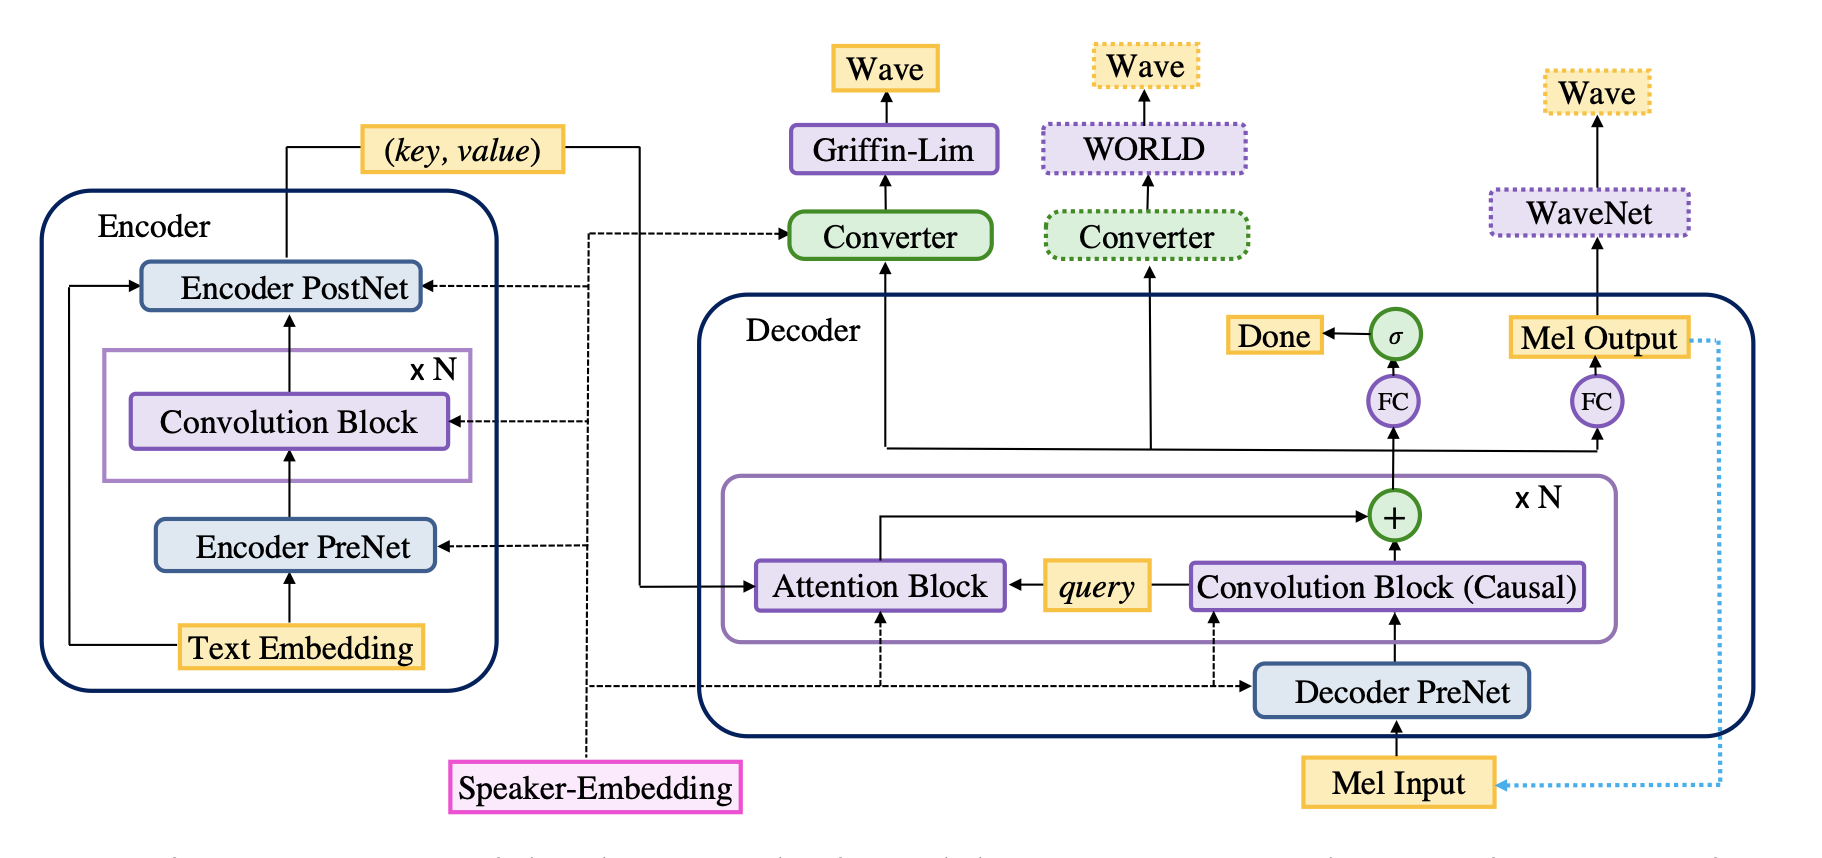
\includegraphics[width=1.0\textwidth]{images/related-work/deepvoice-3.png}
\caption{Encoder-decoder структура в архитектуре DeepVoice3}
\label{fig:related-work:deepvoice-3}
\end{figure}

\begin{figure}[!ht]
\centering
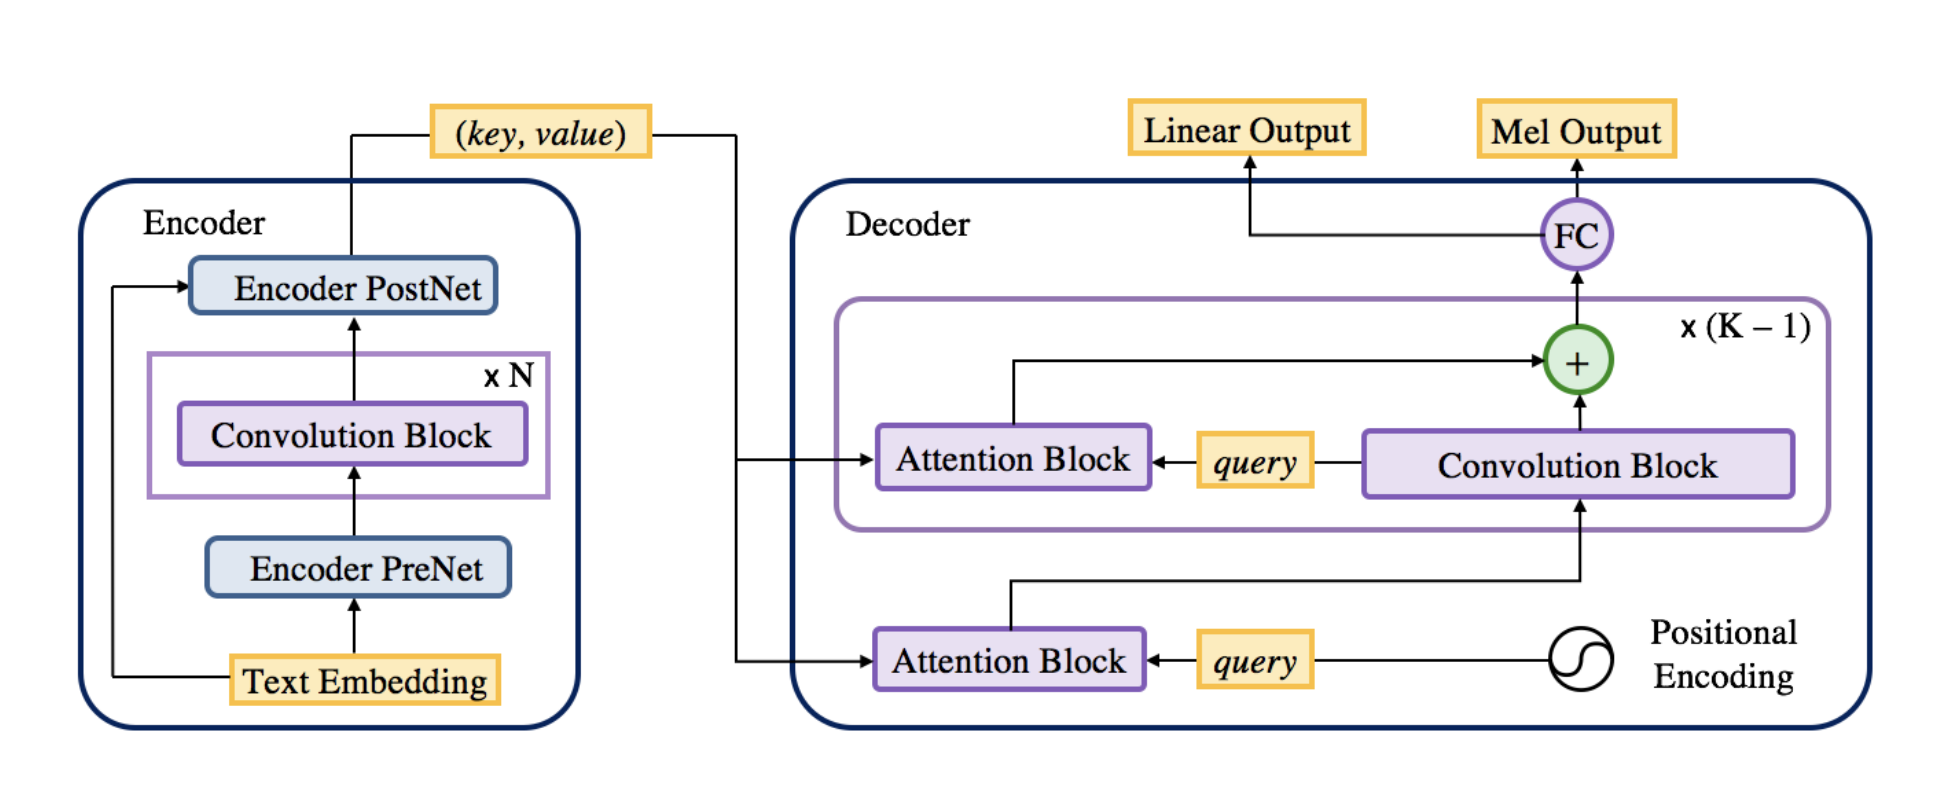
\includegraphics[width=1.0\textwidth]{images/related-work/paranet.png}
\caption{Архитектура ParaNet~\cite{paranet}}
\label{fig:related-work:paranet}
\end{figure}

\begin{figure}[!ht]
\centering
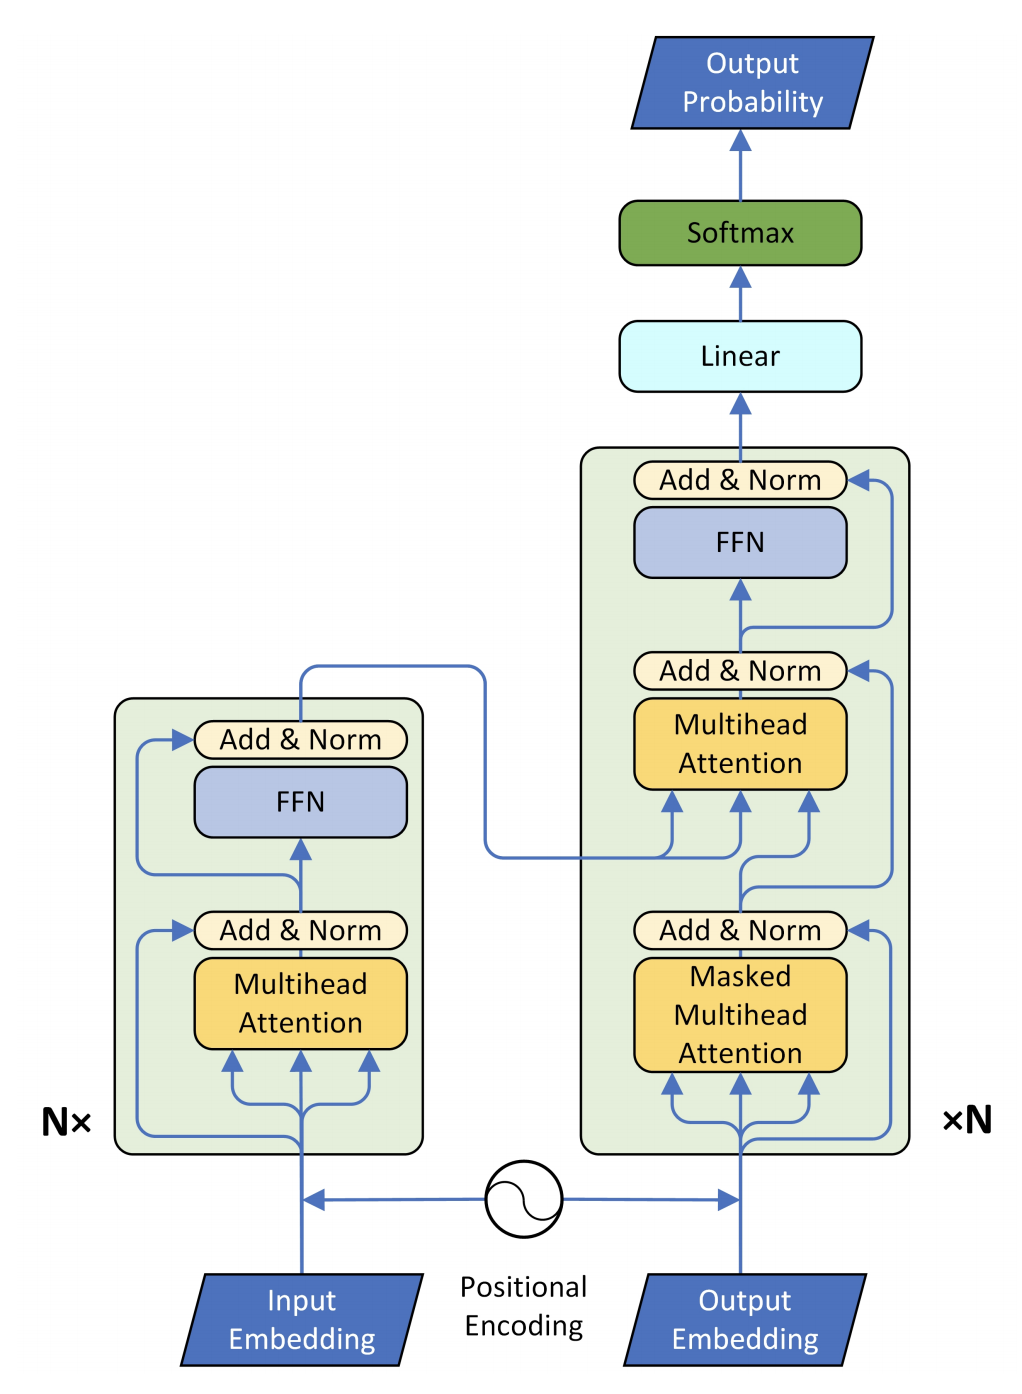
\includegraphics[width=0.7\textwidth]{images/related-work/transformer-tts.png}
\caption{Encoder-decoder Архитектура Transformer-TTS~\cite{transformer-tts}}
\label{fig:related-work:transformer-tts}
\end{figure}

Как и в других моделях, основанных на внимании, Tacotron, Transformer-TTS и ParaNet иногда пропускают или повторяют слова~\cite{paranet}. Чтобы предотвратить пропуск и повторение слов, FastSpeech~\cite{fastspeech} предлагает end-to-end модель с использованием трансформеров~\cite{attention-is-all} взамен традиционной структуре encoder-attention-decoder. FastSpeech использует явный регулятор длины в виде отдельного декодера, который расширяет последовательность фонем в соответствии с предсказанной длительностью, чтобы длина последовательности стала соответствовать длине мэл-спектро\-граммы. Длительности фонем извлекается из выравнивания механизма внимания во внешней предварительно обученной модели TTS, Tacotron 2.
Такой подход показывает неплохие результаты с точки зрения качества и значительно повышает скорость генерации. FastSpeech -- первая модель, показавшая, что идею с промежуточным шагов предсказания длительностей можно успешно применять для построения хорошо работающей TTS системы. Во многом, результаты текущей работы, основаны на продолжении и развитии идей FastSpeech.

\begin{figure}[!ht]
\centering
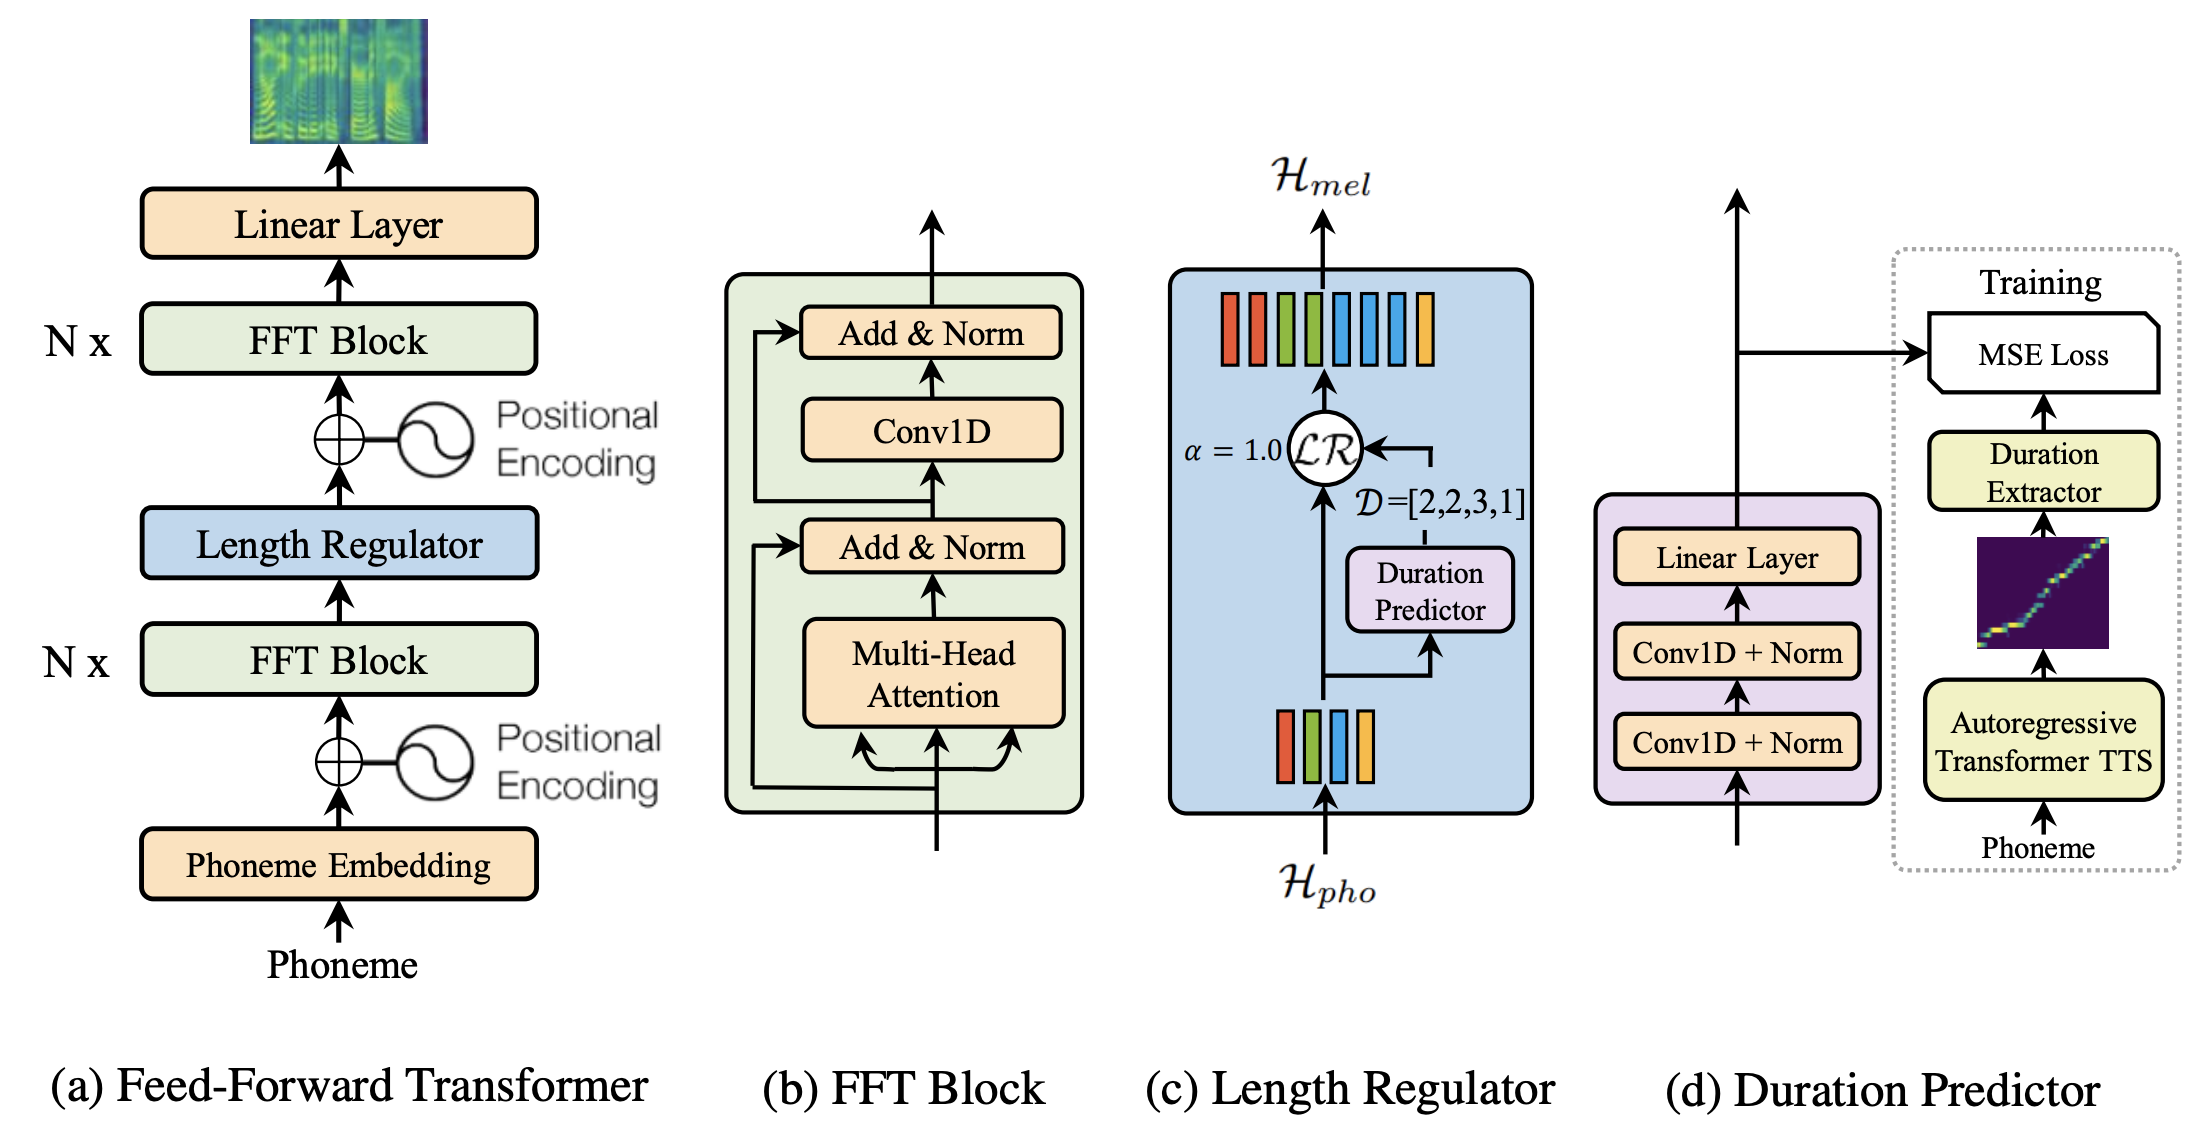
\includegraphics[width=1.0\textwidth]{images/related-work/fastspeech.png}
\caption{Архитектура FastSpeech~\cite{fastspeech}}
\label{fig:related-work:fastspeech}
\end{figure}

Как видно, идеи из области глубокого обучения позволили успростить подходы для генерации речи.